\chapter{La description du carrefour}

% Introduction du chapitre

% Questions soulevées:
% - Pourquoi vouloir décrire le carrefour ?
% - Comment décrire une donnée géographique ?
% - Quels textes veut-on générer ? Pour quels dispositifs ?

Les descriptions textuelles et verbales font partie des outils mobilisés par les personnes concernées par la déficience visuelle pour effectuer un déplacement. Ces descriptions peuvent provenir de dispositifs de guidage, comme une application mobile, et être générées en cours de trajet et lue par synthèse vocale. Bien qu’utilisés par une partie des concernés ([x]\% d’après \cite{homere_2023}), ces dispositifs sont rarement pleinement satisfaisants à cause d’une localisation imprécise et d’informations piétonnes manquantes \missref{}. Au niveau des carrefours notamment, ces imprécisions ne permettent pas de guider une personne de manière sécurisée, en décrivant intégralement une traversée et la qualité de son équipement. Pour un besoin spécifique et sur un itinéraire donné, un \gls{ia} peut préparer manuellement une description, dont le niveau de détails pourra par ailleurs être adapté aux besoins de la personne destinataire, et intégrer toutes les informations nécessaires en se basant sur sa connaissance du terrain. La réalisation d’une telle description est, en revanche, particulièrement chronophage, car elle est spécifique à chaque terrain étudié et chaque besoin \missref{}.

\newpar{}

Pour répondre à cette problématique, dans ce chapitre, nous allons nous intéresser à la manière de réaliser une description de manière semi-automatique en se basant sur des données géographiques. Nous présenterons dans un premier temps le processus général, fortement basé sur les capacités d’un Système d’Information Géographique et nécessitant par conséquent des connaissances spécifiques, puis nous montrerons son application à différents cas d’usages qui peuvent aller au-delà du texte linéaire.


\section{Des données géographiques au texte}

\label{sec:description_geodata_to_text}

Nous avons vu dans le chapitre \ref{chap:modelisation} qu’il pouvait exister des données suffisamment complètes pour proposer une modélisation du carrefour. Cette modélisation peut avoir des applications multiples (voir chapitre 4) dont la génération d’une description textuelle de celui-ci en suivant une approche données vers texte \cite{reiter-2007-architecture}. Cette approche a notamment été suivie par \missref{} et \missref{} pour produire des descriptions de carrefours et de leurs traversées, mais en utilisant des données conçues à cet effet et non des données issues d’une base de données publiques. Par ailleurs, les descriptions proposées sont figées, adaptées à un contexte unique qui ne correspond pas forcément à la variété des besoins exprimés par les instructeurs pour l’autonomie et les personnes concernées. Au-delà du carrefour, des besoins spécifiques peuvent impliquer la modulation du texte (vocabulaire, verbosité) pour réduire la charge cognitive \missref{}, mais également l’intégration de données nouvelles pour décrire des éléments extérieurs à la voirie (par exemple, les arrêts de bus). Ainsi, nous souhaitons proposer un outil flexible qui permettrait à l’instructeur de concevoir une description selon les besoins exprimés et de générer le texte correspondant sur différentes localisations. L’ajout de données arbitraires amène à généraliser le problème à la création d’un texte depuis toute donnée géographique.

\newpar{}

Plusieurs problématiques émergent cependant de cette possibilité : au sujet des carrefours, les chapitres \ref{chap:modelisation} et \ref{chap:evaluation} montrent que les données ou les résultats des traitements algorithmiques sur celles-ci sont parfois incomplets ou incorrects et peuvent nécessiter une correction. Par ailleurs, toute donnée n’est pas nécessairement adaptée à une verbalisation et peut nécessiter un traitement en amont pour la textualiser, à l’instar des traitements réalisés sur une donnée pour la cartographier \missref{}. Ces traitements sont généralement réalisés au sein d’un Système d’Information Géographique par un cartographe ou un géomaticien, or les instructeurs pour l’autonomie comme les adaptateurs-transcripteurs n’ont généralement pas les connaissances pour manipuler ces outils. Pour répondre à ces problématiques, nous proposons d’ajouter le géomaticien comme intermédiaire supplémentaire à la chaîne de génération de description. Ce dernier sera ainsi l’utilisateur principal de l’outil proposé et pourra intégrer les besoins des différentes parties au sein d’une chaîne de traitements de données géographiques permettant de générer du texte.

\subsection{Définition de la description}

Pour lire des documents textuels virtuels, les personnes déficientes visuelles utilisent généralement un lecteur d’écran, un logiciel qui retranscrit par synthèse vocale ce qui est affiché sur l’écran du terminal. Une particularité des lecteurs d’écran est qu’ils ne font pas une simple retranscription texte vers voix mais qu’ils retranscrivent aussi la structure du document lu \missref{}. Cela signifie qu’en parcourant le document, la personne sera informée des titres, des paragraphes, des listes, etc. La lecture est par ailleurs interactive : il est possible de sauter un paragraphe, de revenir au précédent, ou encore de parcourir un à un les éléments d’une liste.

\newpar{}

Dans la suite de ce chapitre, une description sera définie par un texte possiblement augmenté \missref{}, c’est à dire un texte dont les élément sont annotés pour enrichir son contenu. Ces annotations permettent notamment la réalisation d’un document structuré mais aussi d’organiser les textes entre eux.

\subsection{Spécification du système de conception de description}

Un Système d’Information Géographique est un système informatique permettant l’acquisition, le stockage, l’interrogation, le traitement, l’analyse, et la visualisation de données géographiques \cite{AschanLeygonie2019}. Il peut s’agir d’un logiciel de bureau utilisable au travers d’une interface graphique ou d’un système architecturé autour d’une base de données spatiales. S’il existe des SIG avec des modes de représentation de la donnée spécifiques \missref{}, le modèle le plus courant consiste en un empilement de couches thématiques : chaque couche étant un fichier indépendant avec ses propres attributs et métadonnées (projection, sémantique, géométrie). On distingue en général les couches de type raster (image multispectrale dont chaque pixel a une valeur) des couches de type vecteur (donnée tabulaire dont un ou plusieurs champs peuvent contenir une géométrie), ces dernières ayant un fonctionnement proche des tables telles qu’elles existent dans les Systèmes de Gestion de Bases de Données Relationnelles. 

\newpar{}

Un des intérêts des SIG concerne la possibilité d’y réaliser des chaînes de traitements, c’est-à-dire une succession de traitements appliqués à un ensemble de données en entrées pour obtenir un nouvel ensemble de données en sorties. Cela peut inclure entre autres des sélections basées sur la sémantique ou la géométrie, des jointures entre couches et des modifications ou des créations de champs attributaires ou géométriques. Ces chaînes permettent de généraliser un traitement complexe pour l’appliquer sur plusieurs ensembles de données et sur plusieurs territoires. À l’instar des traitements qu’elles embarquent, elles peuvent également être paramétriques afin de piloter leur exécution si nécessaire. Des outils se reposant sur ce système de chaînes de traitement SIG ont déjà été proposés par la littérature, par exemple pour réaliser des « cartes à la carte » [Bucher, 2007].

\newpar{}

Le cadre de conception de description que nous proposons se repose sur une chaîne similaire à celle que l’on pourrait mobiliser pour générer une carte. En effet, la réalisation d’une carte repose sur trois grandes étapes : la spécification du style, où l’on détermine la forme que l’on souhaite obtenir, le rendu, où l’on mobilise des outils pour traiter les données, et la visualisation, où l’on exécute la chaîne pour obtenir le résultat final [Christophe, 2016]. La spécification du style correspond ici à la conception du canevas modulaire, c’est-à-dire à la conception du texte que l’on souhaite générer et ses variantes possibles. Le rendu correspond aux traitements qui seront appliqués sur les données pour les adapter au contexte et permettre leur textualisation. Enfin, la visualisation correspond à l’exécution de la chaîne de traitements pour obtenir le résultat. Dans notre cas, plusieurs acteurs seront mobilisés à chaque étape. En effet, on considère que l’\gls{ia} se repose sur un géomaticien pour la conception technique de la chaîne de traitement. En revanche, il conserve un rôle de commanditaire : il doit ainsi avoir une idée précise du résultat souhaité pour en permettre l’implémentation. Ces différentes étapes sont détaillées dans les parties suivantes.

\subsubsection{Conception d'un canevas modulaire}

Cette première étape consiste à définir exactement les besoins, qui vont notamment s’exprimer par la sortie souhaitée. Pour cela, l’\gls{ia} va concevoir les formes de description finales : quels seront les textes et leurs éventuelles variations, quels seront leur agencement et leur mise en forme (voir parties \ref{sec:description_textuelle}, \ref{sec:description_carte} et \ref{sec:description_graphe}).

\newpar{}

Avec cette vision finale de la description, l’instructeur peut déterminer les données nécessaires pour la réaliser la description. Il ne s’agit pas ici de déterminer les données disponibles (qui seront acquises et traitées par un géomaticien en partie 3.1.2.2) mais d’estimer les données thématiques et les attributs nécessaires afin, pour chacune, de définir un patron, c’est-à-dire un texte conditionnel qui pourra varier selon les attributs de la donnée. Par ailleurs, il est possible de définir plusieurs patrons pour une donnée, chacun correspondant à un usage (par exemple un patron synthétique et un patron détaillé). Chaque patron est par ailleurs augmenté d’attributs permettant de le caractériser, dont le choix est à la discrétion de l’instructeur.

\newpar{}

On parle de canevas modulaire car la forme finale de la description n’est pas nécessairement figée et peut varier selon des paramètres définis à la conception. Il peut s’agir lors de l’assemblage du texte final de la sélection de patrons spécifiques et leur ordonnancement, ou de variations sur le vocabulaire.

\newpar{}

La conception du canevas est illustrée en figure \ref{fig:desc_canevas_modulaire}.

\begin{figure}
    \centering
    \resizebox{15cm}{!}{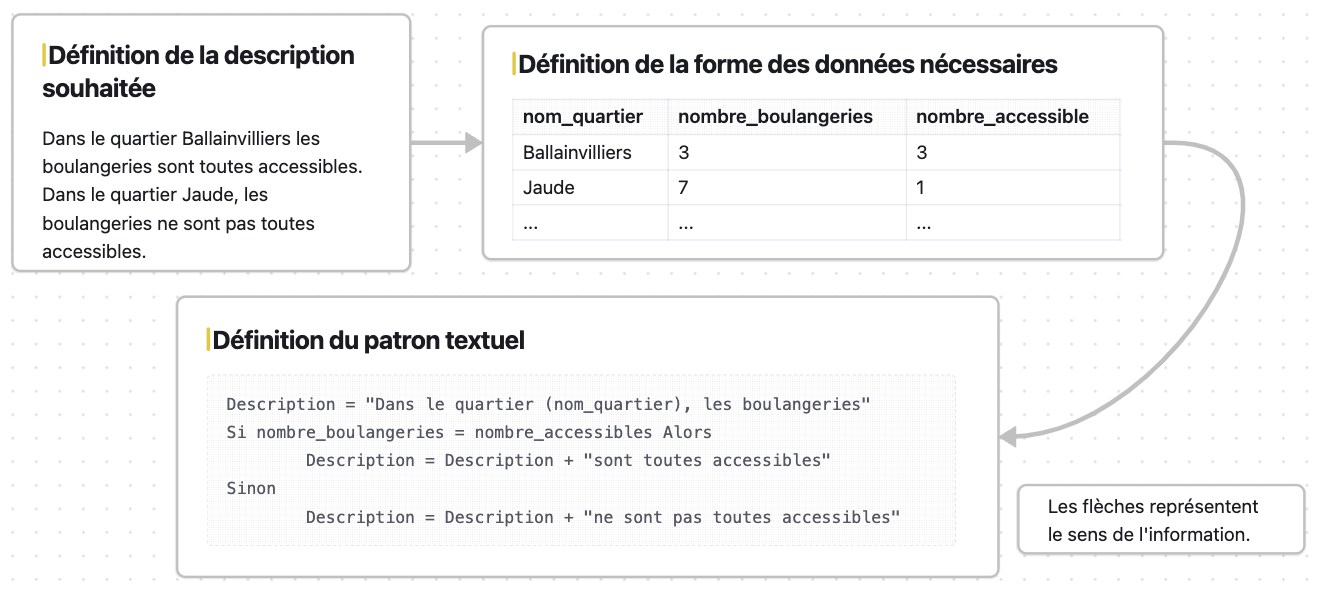
\includegraphics{images/description/conception_canevas.png}}
    \caption{Cet exemple illustre la conception d'un canevas pour générer un résumé par quartier de l'accessibilité des boulangeries.}
    \label{fig:desc_canevas_modulaire}
\end{figure}

\subsubsection{Conception de la chaîne de traitement SIG}

Après la définition du besoin par l’\gls{ia}, le géomaticien a en charge l’implémentation de la chaîne de traitements au sein d’un SIG. Pour cela, il doit tout d’abord identifier et évaluer les sources de données disponibles au regard du besoin. L’évaluation comprend ici la précision des données, qui peut être à la fois la précision métrique mais aussi le niveau de détails (pour un trottoir par exemple, a-t-on besoin de lignes ou de polygones ?) ou encore la couverture géographique (est-ce que la description doit pouvoir s’appliquer partout ou sur un territoire donné ?).

\newpar{}

Une fois les données connues, il peut réaliser la chaîne de traitements SIG qui s’articule autour des trois étapes suivantes :

\begin{enumerate}
    \item \textbf{Traitement des données pour les adapter au contexte}\\
            \textbf{Entrée}: Données géographiques\\
            \textbf{Sortie}: Données géographiques\\
            En ayant maintenant les données à sa disposition, le géomaticien peut utiliser les outils du SIG pour réaliser des traitements sur celles-ci. À l’instar des traitements réalisés pour faire une carte (généralisation géométrique, conception de nouveaux indicateurs) il s’agit ici d’adapter les données à l’usage, ici la réalisation du texte déterminé par les patrons. Cela peut signifier calculer de nouveaux champs, résumer une donnée, réaliser des jointures, etc. Les traitements pourront différer d’une donnée à l’autre et d’une description à l’autre.
    \item \textbf{Implémentation des patrons conçus par l’\gls{ia}}\\
        \textbf{Entrée}: Données géographiques\\
        \textbf{Sortie}: Données géographiques décrites et annotées\\
        Pour chaque entité de chaque couche en entrée, le géomaticien implémente les patrons conçus par l’instructeur en fonction des nouvelles données créées lors de l’étape 1. Il définit également l’ensemble des métadonnées associées aux couche pour permettre leur sélection dans l’étape d’assemblage. 
    \item \textbf{Assemblage des textes en description}\\
        \textbf{Entrée}: Données géographiques décrites et annotées\\
        \textbf{Sortie}: Description\\
        Cette étape correspond à l’assemblage qui va permettre de sélectionner et d’agencer les couches décrites en étape 3 au sein de la description, en accord avec le canevas établi par l’\gls{ia}.
\end{enumerate}

Le processus est illustré en figure \ref{fig:desc_chaine_sig}

\begin{figure}
    \centering
    \resizebox{15cm}{!}{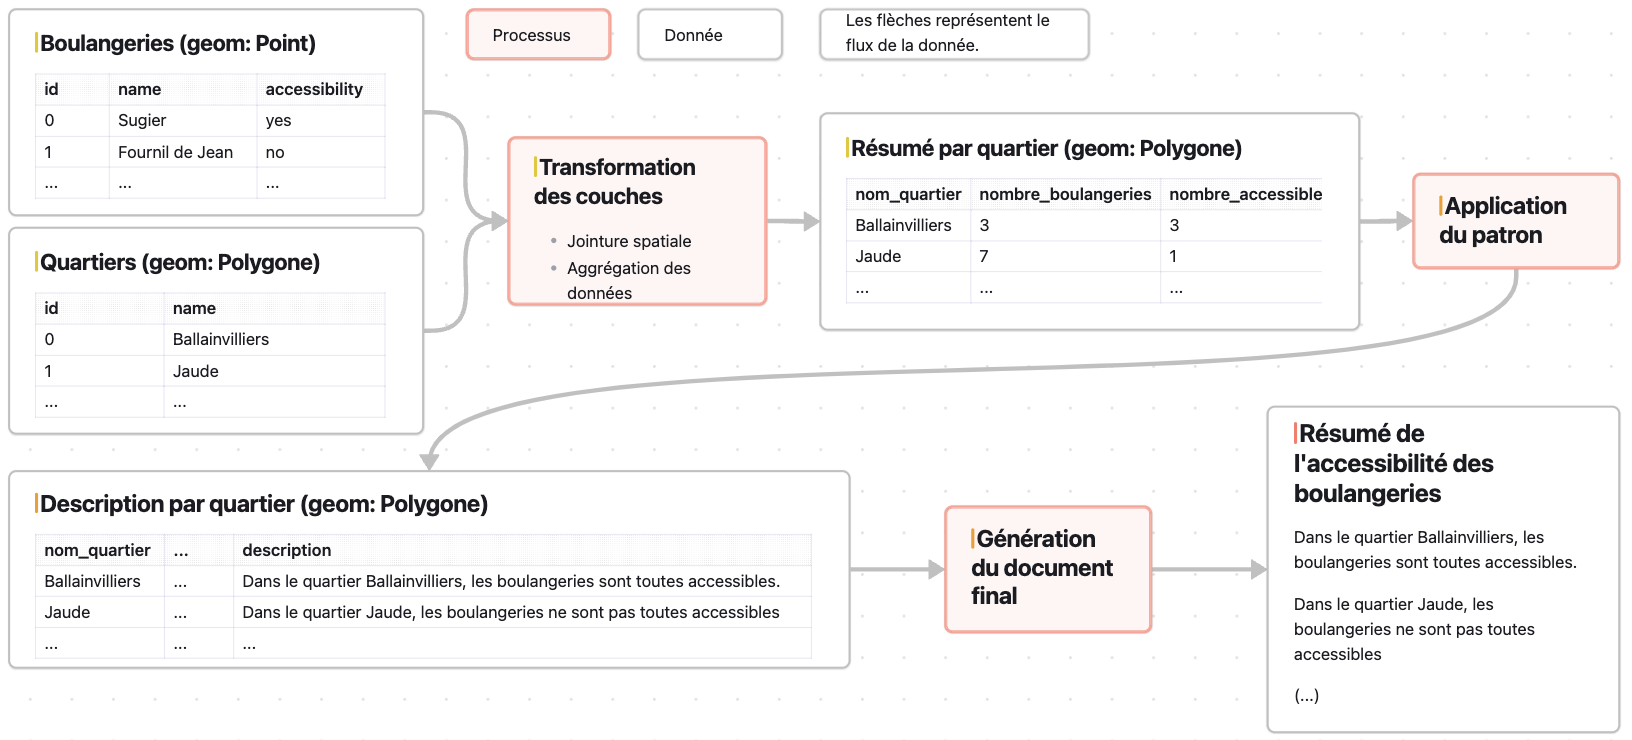
\includegraphics{images/description/conception_pipeline.png}}
    \caption{La chaîne de traitement produite par le géomaticien pour générer l'exemple des boulangeries.}
    \label{fig:desc_chaine_sig}
\end{figure}

\subsubsection{Réalisation d'une description}

L’utilisateur final de l’outil est l’\gls{ia}. Une fois la chaîne réalisée, il va pouvoir la mobiliser sur différents territoires pour générer des descriptions pour les personnes déficientes visuelles avec lesquelles il travaille le déplacement autonome.

\section{Cas d'utilisation: la description des carrefours}

Le cadre présenté en partie \ref{sec:description_geodata_to_text} permet de générer du texte brut ou augmenté depuis toute donnée géographique. S'il permet une application à une diversité de cas d'usage, les notres se concentrent spécifiquement sur la description de carrefour à destination de \gls{pcdv}. Dans cette partie nous nous intéressons à trois applications du cadre présenté à la description de carrefour, dont la variété des objectifs et des supports permettent d'illustrer la souplesse du processus.

\subsection{La réalisation d'une description textuelle}

\label{sec:description_textuelle}

% 1. Définition
On appelle description exocentrée une description dont la position des éléments spatiaux est décrite de manière générale et non relativement à un point donnée.

La lecture d'une description exocentrée est analogue à la lecture d'une carte exocentrée: les informations présentées ne nécessitent pas de traitement en temps réel et sont intrinsèques à l'objet décrit. Cependant, comme présenté dans la partie \ref{sec:description_geodata_to_text}, une description exocentrée ne décrit pas nécessairement des données brutes. Un traitement adapté au texte voulu peut être réalisé sur celles-ci pour intégrer du contexte spatial. Ainsi, il est possible dans une description exocentrée de décrire une relation spatiale ("la boulangerie est dans un quartier") ou une orientation relative aux points cardinaux,.

\newpar{}

Une description égocentrée est une description dont la position des éléments spatiaux est présentée de manière relative à un sujet et écrite à la première personne. Le sujet est placé virtuellement au sein de l'environnement. Le texte peut alors mobiliser des prépositions spatiales telles que "en face", "à droite"...

\subsection{La réalisation d'une description dans la carte}

\label{sec:description_carte}

Une description, si elle conserve des attributs géographiques, peut également être intégrée au sein d'une carte interactive. Si toute carte dématérialisée permet d'embarquer du texte au sein des objets qu'elle représente (généralement accessible par une infobulle), des dispositifs physiques tels que DERi \missref{} permettent de déclencher un son lors de l'appui sur un interacteur. Ainsi, lors de la préparation du canevas modulaire, où pour chaque donnée décrite un texte est associé à chaque entité, il est possible d'intégrer ces entités non-pas au sein d'un document textuel mais d'une carte qui permet d'accéder à la description de chaque entité indépendamment.

\subsection{La réalisation d'une description sous forme de graphe}

\label{sec:description_graphe}

Le cadre défini dans la partie \ref{sec:description_geodata_to_text} présente une description comme un ensemble de textes augmentés pouvant embarquer des informations supplémentaires pouvant permettre une mise en forme élaborée de la description finale. Une des mises en forme possible consiste en la création d'un graphe de textes. En définissant à chaque en ensemble de voisins, il devient possible d'utiliser la description pour représenter topologiquement un environnement (voir figure \ref{fig:desc_graphe_texte}).

\begin{figure}
    \centering
    \resizebox{15cm}{!}{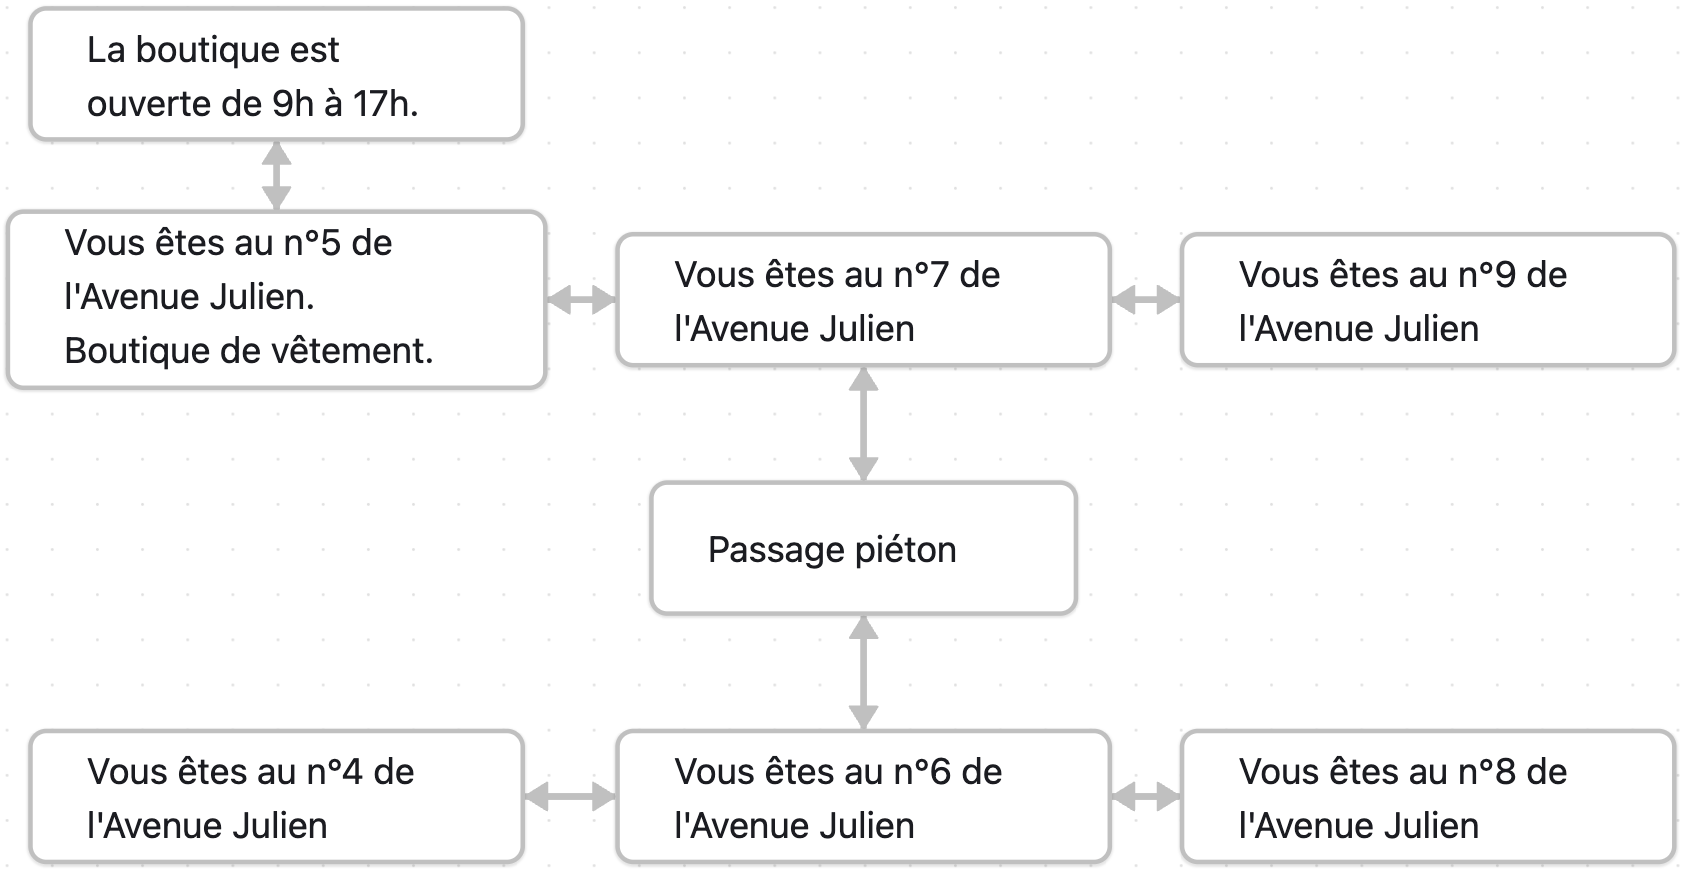
\includegraphics{images/description/graphe_texte.png}}
    \caption{Un graphe de texte permet de représenter un environnement topologique, ici une tronçon de rue. Plusieurs nœuds peuvent dériver d'une même entité géographique (ici une boutique dont les horaire sont indiqués sur un nœud voisin)}.
    \label{fig:desc_graphe_texte}
\end{figure}
\section{Conclusion du chapitre}

Dans ce chapitre, nous avons étudié la problématique de la description textuelle de données géographique, au-delà des carrefours, avec un focus particulier sur l'accessibilité du texte aux \gls{pcdv}. 

\newpar{}

Nous avons proposé un cadre de conception de description intégré à un SIG. Ce cadre propose de partir du besoin exprimé par l'\gls{ia} pour permettre à un géomaticien d'implémenter une chaîne de traitement qui, à partir de données géographiques, réalise la description nécessaire et permet d'appliquer, en fonction de la qualité des données, cette description sur plusieurs territoires. Le besoin de modularité exprimé par les instructeurs est intégré sous la forme de paramètres permettant à l'exécution d'agir sur la description générée: verbosité, vocabulaire, etc. 

\newpar{}

Les outils permettant de réaliser la chaîne de traitement ont été implémentés dans le SIG QGIS et leur fonctionnnement technique est présenté au chapite \ref{chap:implementation}. Par ailleurs, l'évaluation des capacités du dispositif à générer des descriptions effectivement exprimées par des \gls{ia} est présentée en chapitre \ref{chap:evaluation}.